\documentclass{article}
\usepackage{graphicx} % Required for inserting images
\graphicspath{ {../diagram/} }
\usepackage[margin=2cm]{geometry}

\title{DSP in VLSI \\ Homework 1 - Sorter}
\author{Jen-Tse Chen}
\date{March 2026}

\begin{document}
\maketitle

\begin{enumerate}
    \item First, generate several random sequences with 32 elements $[x_1, x_2, \dots, x_{32}]$ in a block between -256 and 255 as your test inputs and prepare as the testbench. (10\%)

    A Python script was used to generate random sequences of 32 elements with values ranging from -256 to 255. These sequences are stored in \texttt{input.txt}. 

    The testbench reads this file to provide a continuous stream of input blocks for the simulation. For the corresponding signal transitions, please refer to the waveforms provided in Figure \ref{fig:SelectTopK_input}.

    \item Please use Verilog to implement \texttt{Sort8} with bitonic sorter. Feed the 8 inputs $[x_1, x_2, \dots, x_8]$ simultaneously in one clock cycle. Observe the outputs to realize sorting among eight elements in one group. Use $[x_1, x_2, \dots, x_8]$ as the input and check for the correctness of the function ``\texttt{Sort8}'', which can generate sorted output from maximum to minimum. Indicate this function output in the timing diagram of your behavior simulation results. (If the data value inside the timing diagram can not be clearly seen, it will not be regarded as correct answers.) (10\%)

    The functional correctness of the \texttt{Sort8} module was verified via behavioral simulation. Eight signed integers were fed simultaneously into the bitonic sorter within a single clock cycle. The simulation output (shown in Figure \ref{fig:Sort8_in_out}) matches the Golden Model generated by the Python script: \texttt{[254, 220, 126, 109, 66, -26, -158, -239]}.
    \begin{figure}
        \centering
        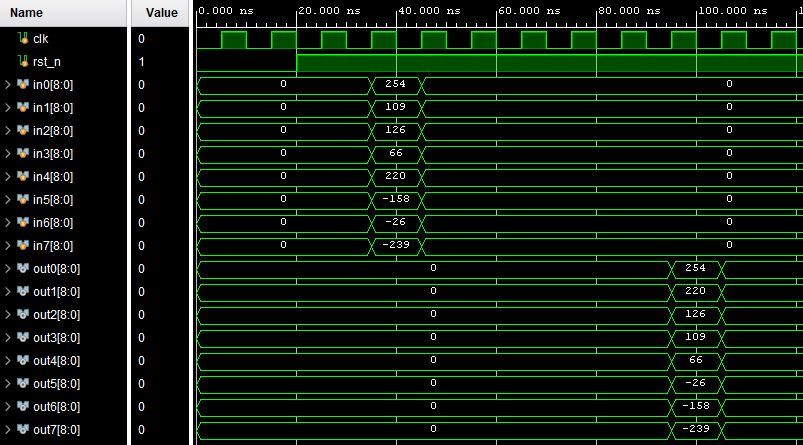
\includegraphics[width=0.8\textwidth]{../diagram/Sort8_input_output.png}
        \caption{Verification of module \texttt{Sort8}}
        \label{fig:Sort8_in_out}
    \end{figure}

    \newpage
    \item Construct the module (\texttt{SelectTopK}) of merger sort to select top 4 among 32 input elements ($[x_1, x_2, x_3, \dots, x_{32}]$) under your control. Use a comparator tree to receive the sorted results from each group and then activate your comparator tree to select top 4 values. Maybe you need two sets of \texttt{Reg8} buffers, one for saving the outputs of the next block from \texttt{Sort8}, and the other for sending the contents of the current block to the comparator tree.\\
    Draw the block diagram of your own implementation and calculate the number of adders/subtractors/comparators in your block diagram. (20\%)\\
    Show the timing diagram of your behavior simulation results (10\%)\\
    Show the hardware output is correct by comparing it to your Matlab results. (10\%)

    The design implements a hierarchical selection network to extract the top-4 elements from 32 inputs. Based on the architectural diagrams (Figures \ref{fig:SelectTopK} through \ref{fig:ComparatorTree}), the hardware resource consumption is as follows:
    \begin{enumerate}
        \item Module \texttt{Sort8} utilizes 24 9-bit comparators (based on the standard $N \log^2(N)$ stages for a bitonic network).
        \item Module of comparator tree used to merge and select the top-4 values consists of 3 9-bit comparators.
        \item The complete module \texttt{SelectTopK} utilizes 27 9-bit comparators.
    \end{enumerate}
    The behavioral simulation results, illustrated in Figure \ref{fig:SelectTopK_input} and Figure \ref{fig:SelectTopK_output}, confirm the module's ability to process 32 elements across four distinct blocks. The hardware output was verified against the Golden Model generated by the Python script:
    \begin{verbatim}
        Block 0: [254 220 174 164]
        Block 1: [248 225 195 189]
        Block 2: [236 235 228 203]
        Block 3: [248 233 219 217]
    \end{verbatim}


    \begin{figure}[h]
        \centering
        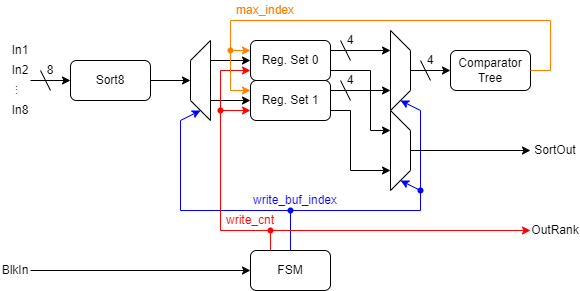
\includegraphics[width=0.8\textwidth]{../diagram/SelectTopK.png}
        \caption{Design of module SelectTopK}
        \label{fig:SelectTopK}
    \end{figure}
    
    \begin{figure}
        \centering
        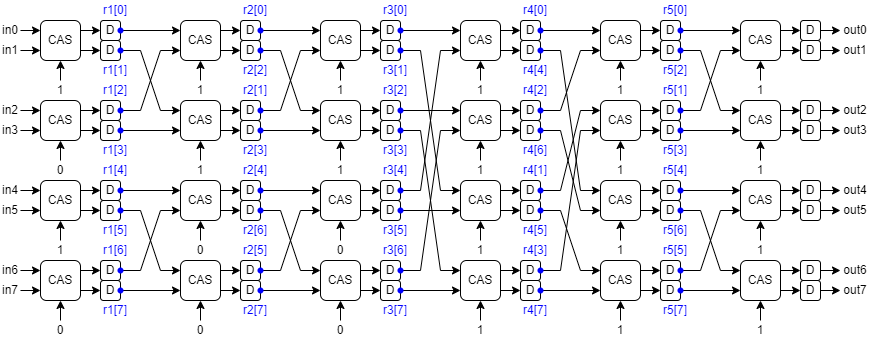
\includegraphics[width=0.8\textwidth]{../diagram/Sort8.png}
        \caption{Design of module \texttt{Sort8} (CAS is Compare And Swap, refer to Figure \ref{fig:CompSwap} for details)}
        \label{fig:Sort8}
    \end{figure}

    \begin{figure}
        \centering
        % Left Column
        \begin{minipage}{0.25\textwidth}
            \centering
            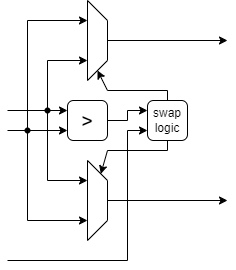
\includegraphics[width=\textwidth]{../diagram/CompSwap.png}
            \caption{Design of module of compare and swap}
            \label{fig:CompSwap}
        \end{minipage}
        % \hfill
        \hspace{1cm}
        % Right Column
        \begin{minipage}{0.4\textwidth}
            \centering
            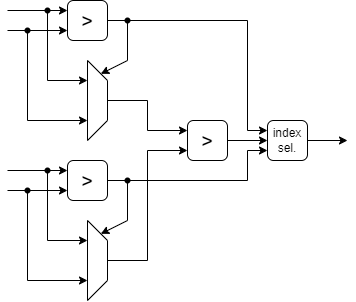
\includegraphics[width=\textwidth]{../diagram/ComparatorTree.png}
            \caption{Design of module of comparator tree}
            \label{fig:ComparatorTree}
        \end{minipage}
    \end{figure}

    \begin{figure}
        \centering
        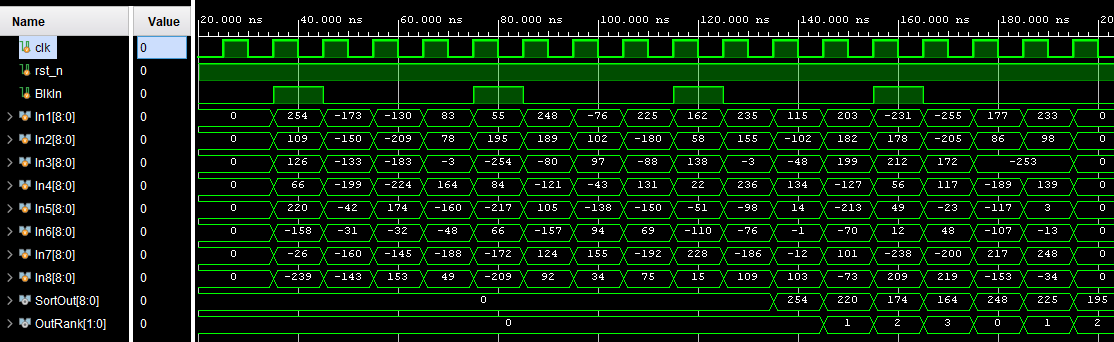
\includegraphics[width=0.8\textwidth]{../diagram/SelectTopK_input.png}
        \caption{Verification input of module \texttt{SelectTopK}}
        \label{fig:SelectTopK_input}
    \end{figure}

    \begin{figure}
        \centering
        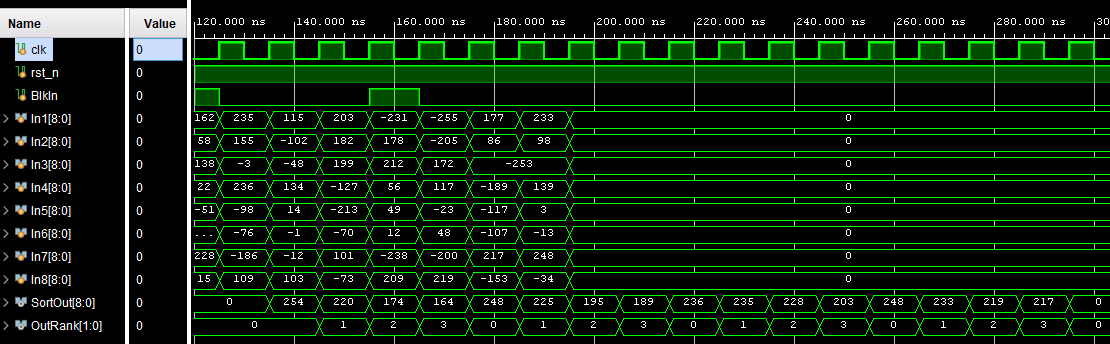
\includegraphics[width=0.8\textwidth]{../diagram/SelectTopK_output.png}
        \caption{Verification output of module \texttt{SelectTopK}}
        \label{fig:SelectTopK_output}
    \end{figure}

    \newpage
    \item Show that your design can generate required top-4 output in descending order every 4 clock cycles with proper input signal ``\texttt{BlkIn}'' and output indicator ``\texttt{OutRank}''. Please feed 4 blocks and check the outputs of four blocks. If it is too long, please cut it down into several segments to make the numerical expressions in the timing diagram clear. If the numerical expressions are hard to distinguish, correct evaluation may not be given. (30\%)

    As shown in Figures \ref{fig:SelectTopK_input} and \ref{fig:SelectTopK_output}, the design successfully generates the top-4 output in descending order every 4 clock cycles. The \texttt{BlkIn} signal effectively triggers block processing, while \texttt{OutRank} correctly identifies the sorted position of each element.

    To sustain continuous streaming input, the design implements:
    \begin{enumerate}
        \item Ping-Pong Buffering: A dual-buffer scheme (Fig. \ref{fig:SelectTopK}) allows simultaneous sorting of new data while selecting the Top-4 from the previous set.
        \item FSM Control: A Finite State Machine (Fig. \ref{fig:FSM}) orchestrates the buffer switching and signal timing, ensuring a seamless transition across the 4-block sequence. Upon receiving the \texttt{BlkIn} signal, the \texttt{blk\_cnt} register increments. Conversely, once a block output operation completes, \texttt{blk\_cnt} decrements. The ping-pong buffering state machine transitions back to IDLE only when \texttt{blk\_cnt} reaches zero.
    \end{enumerate}

    \begin{figure}
        \centering
        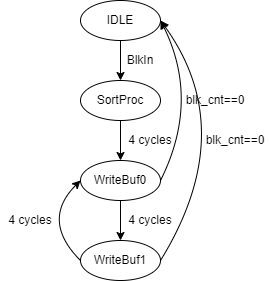
\includegraphics[width=0.4\textwidth]{../diagram/FSM.png}
        \caption{Finite state machine of module \texttt{SelectTopK}}
        \label{fig:FSM}
    \end{figure}

    \newpage
    \item Please use Matlab command ``sort'' to verify your results of your randomly-generated sequence and compare to the Verilog simulation results (10\%).

    The functional correctness of the design is verified against the randomly generated input and the Golden Model described in Q3. Both methods confirm that the hardware output is perfectly aligned with the expected sorted results.

    \item Synthesis your design in Q4. Show the number of adders/subtractors/ comparators in your design. Sum them up together to see if it matches with your block diagram. (10\%) (Because you may use counters to control your circuits, we will not ask that the two values should be exactly the same. However, there should not be a large discrepancy.)

    The design was synthesized at a clock frequency of 50 MHz. The resulting timing and area reports are provided in Figure \ref{fig:timing_report} and Figure \ref{fig:area_report}, respectively.

    \begin{figure}[h]
        \centering
        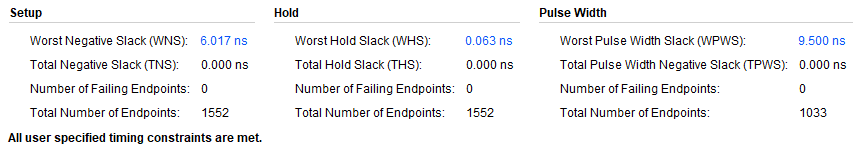
\includegraphics[width=0.8\textwidth]{../diagram/timing_report.png}
        \caption{Timing report}
        \label{fig:timing_report}
    \end{figure}

    \begin{figure}
        \centering
        
\includegraphics[width=0.8\textwidth]{../diagram/area_report.png}
        \caption{Area report}
        \label{fig:area_report}
    \end{figure}

    \newpage
    The architectural design specifies 27 9-bit comparators (24 within the \texttt{Sort8} module and 3 within the module of comparator tree). In the targeted FPGA architecture, a single 9-bit signed comparison typically maps to 2 \texttt{CARRY4} primitives. The synthesis report indicates a total usage of 54 \texttt{CARRY4} blocks. This matches the expected consumption, confirming that the synthesizer preserved the intended logic structure without significant discrepancy.
    \begin{verbatim}
        +----------+------+---------------------+
        | Ref Name | Used | Functional Category |
        +----------+------+---------------------+
        | FDCE     | 1030 |        Flop & Latch |
        | LUT3     |  447 |                 LUT |
        | LUT4     |  444 |                 LUT |
        | LUT6     |  237 |                 LUT |
        | LUT5     |   83 |                 LUT |
        | IBUF     |   75 |                  IO |
        | MUXF7    |   70 |               MuxFx |
        | LUT2     |   62 |                 LUT |
        | CARRY4   |   54 |          CarryLogic |
        | MUXF8    |   35 |               MuxFx |
        | OBUF     |   11 |                  IO |
        | FDPE     |    2 |        Flop & Latch |
        | LUT1     |    1 |                 LUT |
        | BUFG     |    1 |               Clock |
        +----------+------+---------------------+
    \end{verbatim}
    
    
\end{enumerate}

\end{document}
